%==============================================================================
% Deep Reinforcement Learning for Portfolio Optimization
% Main Document - IEDA4000F Final Project Report
%==============================================================================

\documentclass[12pt, a4paper]{article}

% Packages
\usepackage[utf8]{inputenc}
\usepackage[T1]{fontenc}
\usepackage{amsmath, amssymb, amsfonts}
\usepackage{graphicx}
\usepackage{booktabs}
\usepackage{longtable}
\usepackage{geometry}
\usepackage{hyperref}
\usepackage{xcolor}
\usepackage{listings}
\usepackage{algorithm}
\usepackage{algpseudocode}
\usepackage{tikz}
\usepackage{pgfplots}
\usepackage{float}
\usepackage{subcaption}
\usepackage{enumitem}
\usepackage{fancyhdr}
\usepackage{setspace}
\usepackage[numbers]{natbib}
\usepackage{appendix}
\usepackage{multirow}

% Page setup
\geometry{margin=1in, headheight=15pt}
\pgfplotsset{compat=1.18}
\usetikzlibrary{positioning, arrows.meta, shapes.geometric}

% Hyperlink setup
\hypersetup{
    colorlinks=true,
    linkcolor=blue,
    filecolor=magenta,
    urlcolor=cyan,
    citecolor=green!50!black
}

% Header/Footer
\pagestyle{fancy}
\fancyhf{}
\rhead{DRL Portfolio Optimization}
\lhead{IEDA4000F}
\rfoot{Page \thepage}

% Code listing style
\lstset{
    language=Python,
    basicstyle=\ttfamily\small,
    keywordstyle=\color{blue},
    commentstyle=\color{green!60!black},
    stringstyle=\color{red},
    showstringspaces=false,
    breaklines=true,
    frame=single,
    backgroundcolor=\color{gray!10}
}

% Custom commands
\newcommand{\E}{\mathbb{E}}
\newcommand{\R}{\mathbb{R}}
\newcommand{\bw}{\mathbf{w}}
\newcommand{\br}{\mathbf{r}}
\newcommand{\bs}{\mathbf{s}}
\newcommand{\ba}{\mathbf{a}}

%==============================================================================
\begin{document}
%==============================================================================

% Title Page
\begin{titlepage}
\centering
\vspace*{2cm}
{\Huge\bfseries Deep Reinforcement Learning for Portfolio Optimization with Options Hedging\par}
\vspace{1.5cm}
{\Large\itshape IEDA4000F Final Project Report\par}
\vspace{2cm}
{\large CHONG Tin Tak\par}
{\large 20920359\par}
\vspace{1cm}
{\large Department of Industrial Engineering and Decision Analytics\par}
{\large The Hong Kong University of Science and Technology\par}
\vfill
{\large \today\par}
\end{titlepage}

% Abstract
\begin{abstract}
This project investigates the application of Deep Reinforcement Learning (DRL) to portfolio optimization with integrated options hedging and systematic risk management. We implement and compare two state-of-the-art algorithms---Deep Deterministic Policy Gradient (DDPG) and Proximal Policy Optimization (PPO)---for continuous portfolio weight allocation across 18 diversified assets spanning eight market sectors.

Our framework incorporates Black-Scholes options pricing for dynamic hedging and a tiered stop-loss mechanism for systematic downside protection. Training on 2010-2018 market data and testing on 2019-2020 (including the COVID-19 market crash), we find that DDPG significantly outperforms PPO with a Sharpe ratio of 5.52 versus 1.85, achieving 219\% total return while limiting maximum drawdown to just 8.31\% compared to the market's 34\% decline.

DDPG's superior performance stems from its off-policy learning capability and deterministic policy output, which proves advantageous for the portfolio allocation task. The agent learned effective hedging strategies, generating \$126,568 in options profits during the test period. These results demonstrate the practical potential of DRL-based portfolio management for navigating both normal market conditions and tail risk events.

\textbf{Keywords:} Deep Reinforcement Learning, Portfolio Optimization, DDPG, PPO, Options Hedging, Risk Management, COVID-19
\end{abstract}

\newpage
\tableofcontents
\newpage
\listoffigures
\listoftables
\newpage

% Main Sections
\section{Introduction}
\label{sec:introduction}

\subsection{Background and Motivation}

Portfolio optimization has been a cornerstone of modern finance since Harry Markowitz's seminal work on mean-variance optimization in 1952 \cite{markowitz1952}. Traditional approaches rely on statistical estimates of expected returns and covariances, which often prove unstable in practice due to estimation errors that compound over time. These classical methods also struggle to adapt to non-stationary market dynamics and fail to capture complex nonlinear relationships between assets.

The financial markets of the 21st century present unique challenges that expose the limitations of traditional portfolio management approaches:

\begin{itemize}
    \item \textbf{Market Complexity}: Modern markets exhibit intricate dependencies, regime changes, and fat-tailed return distributions that violate the Gaussian assumptions underlying classical models.
    
    \item \textbf{High-Frequency Dynamics}: Rapid information dissemination and algorithmic trading create fast-moving market conditions that require adaptive strategies.
    
    \item \textbf{Tail Risk Events}: Events like the 2008 financial crisis and the COVID-19 market crash of 2020 demonstrate the importance of robust risk management beyond traditional volatility measures.
    
    \item \textbf{Transaction Costs and Constraints}: Real-world portfolio management must account for transaction costs, position limits, and regulatory constraints that classical models often ignore.
\end{itemize}

Deep Reinforcement Learning (DRL) offers a promising alternative framework for portfolio optimization. By framing portfolio management as a sequential decision-making problem, DRL agents can learn adaptive strategies directly from market data without relying on explicit statistical models. Recent advances in deep learning provide the representational capacity to capture complex market patterns, while reinforcement learning algorithms enable optimization of long-term risk-adjusted returns.

\subsection{Research Objectives}

This project investigates the application of Deep Reinforcement Learning to portfolio optimization with the following primary objectives:

\begin{enumerate}
    \item \textbf{Algorithm Comparison}: Implement and compare two state-of-the-art DRL algorithms—Deep Deterministic Policy Gradient (DDPG) and Proximal Policy Optimization (PPO)—for continuous portfolio weight allocation under unified hyperparameters.
    
    \item \textbf{Risk Management Design}: Develop a comprehensive risk management framework combining volatility targeting, progressive position reduction, and aggressive drawdown penalties to achieve $<$10\% maximum drawdown.
    
    \item \textbf{Drawdown Control}: Design and evaluate mechanisms that adapt portfolio exposure based on drawdown levels and realized volatility, providing systematic risk control.
    
    \item \textbf{Stress Testing}: Evaluate the trained agents' performance during extreme market conditions, specifically the COVID-19 market crash of March 2020, to validate the risk management framework.
    
    \item \textbf{Reproducibility}: Create a comprehensive, well-documented codebase that enables reproduction and extension of our results.
\end{enumerate}

\subsection{Key Contributions}

This work makes the following contributions to the field of algorithmic portfolio management:

\begin{enumerate}
    \item \textbf{Volatility Targeting Framework}: We implement industry-standard volatility targeting that scales portfolio exposure based on realized volatility, maintaining consistent risk regardless of market conditions.
    
    \item \textbf{Aggressive Drawdown Control}: We design a multi-layered drawdown control system combining progressive position reduction (starting at 3\% drawdown) with aggressive reward penalties ($\lambda=5.0$) to achieve $<$10\% maximum drawdown target.
    
    \item \textbf{Fair Algorithm Comparison}: We conduct rigorous comparison of DDPG and PPO under unified hyperparameters, demonstrating that both algorithms achieve comparable performance when properly configured.
    
    \item \textbf{COVID-19 Stress Test}: We validate the framework during the March 2020 market crash, demonstrating $<$10\% drawdown while the market declined 33.9\%.
    
    \item \textbf{Open-Source Implementation}: We provide a complete, modular implementation suitable for research and practical applications, including data loading, environment simulation, agent training, and performance visualization.
\end{enumerate}

\subsection{Report Structure}

The remainder of this report is organized as follows:

\begin{itemize}
    \item \textbf{Section \ref{sec:literature}}: Reviews related work in portfolio optimization, reinforcement learning for finance, and options-based hedging strategies.
    
    \item \textbf{Section \ref{sec:methodology}}: Presents the mathematical framework, including the MDP formulation, reward function design, and the DDPG and PPO algorithms.
    
    \item \textbf{Section \ref{sec:implementation}}: Describes the system architecture, code structure, and implementation details.
    
    \item \textbf{Section \ref{sec:experiments}}: Details the experimental setup, including asset selection, data preprocessing, and hyperparameter configurations.
    
    \item \textbf{Section \ref{sec:results}}: Presents comprehensive results comparing DDPG and PPO performance across multiple metrics.
    
    \item \textbf{Section \ref{sec:discussion}}: Analyzes the results, discusses the strengths and limitations of each approach, and provides insights into the learned strategies.
    
    \item \textbf{Section \ref{sec:conclusion}}: Summarizes our findings and outlines directions for future research.
\end{itemize}

Appendices provide detailed mathematical formulas (Appendix \ref{app:formulas}) and configuration parameters (Appendix \ref{app:config}).

\section{Literature Review}
\label{sec:literature}

\subsection{Classical Portfolio Optimization}

The foundation of modern portfolio theory was established by Harry Markowitz \cite{markowitz1952}, who formulated the mean-variance optimization problem. Given $n$ assets with expected returns $\bm{\mu} \in \R^n$ and covariance matrix $\bm{\Sigma} \in \R^{n \times n}$, the investor seeks portfolio weights $\bw \in \R^n$ that maximize expected return for a given level of risk:

\begin{equation}
\max_{\bw} \quad \bw^\top \bm{\mu} - \frac{\lambda}{2} \bw^\top \bm{\Sigma} \bw
\quad \text{s.t.} \quad \bw^\top \mathbf{1} = 1, \quad \bw \geq 0
\end{equation}

where $\lambda$ is the risk aversion parameter. Despite its theoretical elegance, mean-variance optimization suffers from several practical limitations:

\begin{itemize}
    \item \textbf{Estimation Sensitivity}: Small errors in $\bm{\mu}$ and $\bm{\Sigma}$ estimates lead to dramatically different optimal portfolios \cite{michaud1989}.
    \item \textbf{Static Nature}: The single-period formulation ignores the dynamic nature of portfolio rebalancing.
    \item \textbf{Distributional Assumptions}: Gaussian returns assumption fails to capture fat tails and asymmetric distributions observed in financial markets.
\end{itemize}

Extensions such as Black-Litterman \cite{black1992} and robust optimization \cite{goldfarb2003} address some of these limitations but remain fundamentally constrained by their reliance on statistical estimation.

\subsection{Reinforcement Learning Foundations}

Reinforcement learning (RL) provides a framework for sequential decision-making under uncertainty \cite{sutton2018}. An RL agent interacts with an environment modeled as a Markov Decision Process (MDP) defined by the tuple $(\mathcal{S}, \mathcal{A}, P, R, \gamma)$:

\begin{itemize}
    \item $\mathcal{S}$: State space (market observations)
    \item $\mathcal{A}$: Action space (portfolio weights)
    \item $P(s'|s,a)$: Transition dynamics
    \item $R(s,a,s')$: Reward function
    \item $\gamma \in [0,1]$: Discount factor
\end{itemize}

The goal is to find a policy $\pi: \mathcal{S} \rightarrow \mathcal{A}$ that maximizes expected cumulative discounted rewards:

\begin{equation}
J(\pi) = \E_{\pi} \left[ \sum_{t=0}^{\infty} \gamma^t R_t \right]
\end{equation}

\subsection{Deep Reinforcement Learning for Finance}

The application of deep reinforcement learning to financial problems has gained significant momentum in recent years. Several key works have demonstrated the potential of DRL for portfolio management:

\textbf{Jiang et al. (2017)} \cite{jiang2017} proposed a deep learning framework for portfolio management using a convolutional neural network to extract features from historical price data. Their approach achieved competitive performance against traditional benchmarks.

\textbf{Liang et al. (2018)} \cite{liang2018} applied DDPG to portfolio optimization, demonstrating superior performance compared to traditional methods on Chinese stock market data.

\textbf{Yang et al. (2020)} \cite{yang2020} developed FinRL, an open-source library for financial reinforcement learning that provides standardized implementations of popular DRL algorithms.

\textbf{Liu et al. (2021)} \cite{liu2021} proposed an ensemble method combining multiple DRL agents for more robust portfolio decisions.

\subsection{Actor-Critic Methods}

Actor-critic methods combine value-based and policy-based approaches, using a critic to estimate value functions and an actor to optimize the policy. This architecture offers several advantages:

\begin{itemize}
    \item \textbf{Reduced Variance}: The critic's value estimates provide a baseline for variance reduction in policy gradient updates.
    \item \textbf{Continuous Actions}: Actor networks can directly output continuous actions, suitable for portfolio weight allocation.
    \item \textbf{Sample Efficiency}: Combining on-policy and off-policy learning improves data utilization.
\end{itemize}

\subsubsection{Deep Deterministic Policy Gradient (DDPG)}

DDPG \cite{lillicrap2015} extends the deterministic policy gradient theorem to deep neural networks. Key features include:

\begin{itemize}
    \item \textbf{Deterministic Policy}: The actor outputs a deterministic action $a = \mu_\theta(s)$, with exploration noise added during training.
    \item \textbf{Experience Replay}: Transitions are stored in a replay buffer and sampled randomly for training, breaking temporal correlations.
    \item \textbf{Target Networks}: Slowly-updated target networks stabilize training by providing consistent targets for Q-value estimation.
    \item \textbf{Off-Policy Learning}: DDPG can learn from past experiences, improving sample efficiency.
\end{itemize}

\subsubsection{Proximal Policy Optimization (PPO)}

PPO \cite{schulman2017} addresses the challenge of stable policy updates in on-policy methods. Key innovations include:

\begin{itemize}
    \item \textbf{Clipped Objective}: The surrogate objective is clipped to prevent excessively large policy updates.
    \item \textbf{Trust Region}: The clipping mechanism implicitly enforces a trust region constraint on policy changes.
    \item \textbf{Sample Efficiency}: Multiple epochs of optimization on the same batch of data improve learning efficiency.
    \item \textbf{Simplicity}: PPO achieves competitive performance with simpler implementation compared to methods like TRPO.
\end{itemize}

\subsection{Options in Portfolio Management}

Options provide non-linear payoff profiles that can be used for hedging and speculation. The Black-Scholes model \cite{black1973} provides the foundational framework for options pricing:

\begin{equation}
C = S_0 N(d_1) - K e^{-rT} N(d_2)
\end{equation}

where:
\begin{itemize}
    \item $d_1 = \frac{\ln(S_0/K) + (r + \sigma^2/2)T}{\sigma\sqrt{T}}$
    \item $d_2 = d_1 - \sigma\sqrt{T}$
    \item $N(\cdot)$ is the cumulative standard normal distribution
\end{itemize}

Protective puts represent a fundamental hedging strategy where an investor holding a long position purchases put options to limit downside risk. The payoff at expiration is:

\begin{equation}
\text{Payoff} = \max(S_T, K) - P_0
\end{equation}

where $P_0$ is the premium paid for the put option. This creates an asymmetric payoff profile that preserves upside potential while limiting losses.

\subsection{Risk Management in Algorithmic Trading}

Effective risk management is crucial for algorithmic trading systems. Common approaches include:

\begin{itemize}
    \item \textbf{Position Sizing}: Kelly criterion and fractional Kelly methods optimize position sizes based on edge and variance.
    \item \textbf{Stop-Loss Orders}: Automatic position liquidation when losses exceed predetermined thresholds.
    \item \textbf{Portfolio Constraints}: Limits on sector exposure, single-stock concentration, and leverage.
    \item \textbf{Value-at-Risk (VaR)}: Statistical measures of potential losses at given confidence levels.
\end{itemize}

Our work integrates multiple risk management approaches within the DRL framework, including options-based hedging and tiered stop-loss mechanisms.

\subsection{Gap in Literature}

While significant progress has been made in applying DRL to portfolio optimization, several gaps remain:

\begin{enumerate}
    \item \textbf{Options Integration}: Most DRL portfolio management studies focus on equity allocation without incorporating derivative instruments for hedging.
    
    \item \textbf{Systematic Risk Management}: Few studies integrate explicit risk management mechanisms within the DRL framework.
    
    \item \textbf{Stress Testing}: Limited evaluation of DRL agents during extreme market events like the COVID-19 crash.
    
    \item \textbf{Algorithm Comparison}: Comprehensive comparisons between DDPG and PPO for portfolio optimization under consistent experimental conditions are scarce.
\end{enumerate}

This work addresses these gaps by developing an integrated framework that combines DRL-based portfolio optimization with options hedging and systematic risk management, evaluated rigorously during both normal and crisis market conditions.

\section{Methodology}
\label{sec:methodology}

\subsection{Problem Formulation}

We formulate portfolio optimization as a Markov Decision Process (MDP), enabling the application of reinforcement learning algorithms. At each time step $t$, the agent observes market conditions, selects portfolio weights, and receives a reward based on portfolio performance.

\subsubsection{State Space}

The state $s_t \in \mathcal{S}$ captures relevant market information at time $t$:

\begin{equation}
s_t = \begin{bmatrix}
\br_{t-L:t}^\top & \text{vol}_{t-L:t}^\top & \bw_{t-1}^\top & \text{features}_t^\top
\end{bmatrix}
\end{equation}

where:
\begin{itemize}
    \item $\br_{t-L:t} \in \R^{n \times L}$: Historical returns for $n$ assets over lookback window $L$
    \item $\text{vol}_{t-L:t} \in \R^{n \times L}$: Rolling volatility estimates
    \item $\bw_{t-1} \in \R^n$: Current portfolio weights
    \item $\text{features}_t$: Additional technical indicators (momentum, RSI, etc.)
\end{itemize}

The state representation enables the agent to learn patterns from historical price movements while maintaining awareness of current portfolio positioning.

\subsubsection{Action Space}

The action $\ba_t \in \mathcal{A}$ represents the target portfolio allocation:

\begin{equation}
\ba_t = \begin{bmatrix} w_1^t & w_2^t & \cdots & w_n^t & h_t \end{bmatrix}
\end{equation}

Subject to constraints:
\begin{align}
\sum_{i=1}^{n} w_i^t &\leq 1 \quad \text{(allocation constraint)} \\
w_i^t &\geq 0 \quad \forall i \quad \text{(long-only constraint)} \\
h_t &\in [0, h_{\max}] \quad \text{(hedge ratio constraint)}
\end{align}

The hedge ratio $h_t$ determines the fraction of portfolio value allocated to protective put options. Any unallocated capital ($1 - \sum_i w_i^t$) earns the risk-free rate.

\subsubsection{Reward Function}

The reward function balances return maximization with risk management. We use a risk-adjusted reward:

\begin{equation}
r_t = R_t^{\text{port}} - \lambda_{\text{risk}} \cdot \text{Risk}_t - \lambda_{\text{tc}} \cdot \text{TC}_t
\end{equation}

where:

\textbf{Portfolio Return:}
\begin{equation}
R_t^{\text{port}} = \sum_{i=1}^{n} w_i^{t-1} \cdot r_i^t + (1 - \sum_i w_i^{t-1}) \cdot r_f + \Pi_t^{\text{options}}
\end{equation}

\textbf{Risk Penalty:}
\begin{equation}
\text{Risk}_t = \max(0, -R_t^{\text{port}})^2
\end{equation}

\textbf{Transaction Costs:}
\begin{equation}
\text{TC}_t = c \cdot \sum_{i=1}^{n} |w_i^t - w_i^{t-1}|
\end{equation}

The squared downside penalty encourages the agent to avoid large negative returns, while the transaction cost term discourages excessive trading.

\subsection{Deep Deterministic Policy Gradient (DDPG)}

DDPG is an off-policy actor-critic algorithm designed for continuous action spaces. We employ DDPG with the following components:

\subsubsection{Actor Network}

The actor network $\mu_\theta: \mathcal{S} \rightarrow \mathcal{A}$ maps states to deterministic actions:

\begin{equation}
\ba_t = \mu_\theta(s_t)
\end{equation}

Architecture: $\text{State} \rightarrow \text{FC}(256) \rightarrow \text{ReLU} \rightarrow \text{FC}(256) \rightarrow \text{ReLU} \rightarrow \text{FC}(n+1) \rightarrow \text{Softmax}$

The softmax output ensures valid portfolio weights that sum to at most 1.

\subsubsection{Critic Network}

The critic network $Q_\phi: \mathcal{S} \times \mathcal{A} \rightarrow \R$ estimates the Q-value:

\begin{equation}
Q_\phi(s_t, \ba_t) \approx \E\left[\sum_{k=0}^{\infty} \gamma^k r_{t+k} \mid s_t, \ba_t\right]
\end{equation}

Architecture: State and action are concatenated after initial state processing:
\[
\text{State} \rightarrow \text{FC}(256) \rightarrow \text{ReLU} \rightarrow [\cdot, \ba] \rightarrow \text{FC}(256) \rightarrow \text{ReLU} \rightarrow \text{FC}(1)
\]

\subsubsection{Training Algorithm}

DDPG training alternates between:

\textbf{Critic Update:} Minimize temporal difference error:
\begin{equation}
L(\phi) = \E_{(s,a,r,s') \sim \mathcal{D}} \left[ \left( Q_\phi(s,a) - y \right)^2 \right]
\end{equation}

where the target is:
\begin{equation}
y = r + \gamma Q_{\phi'}(s', \mu_{\theta'}(s'))
\end{equation}

\textbf{Actor Update:} Maximize expected Q-value via deterministic policy gradient:
\begin{equation}
\nabla_\theta J = \E_{s \sim \mathcal{D}} \left[ \nabla_a Q_\phi(s,a)|_{a=\mu_\theta(s)} \cdot \nabla_\theta \mu_\theta(s) \right]
\end{equation}

\textbf{Target Network Update:} Soft update with parameter $\tau$:
\begin{align}
\theta' &\leftarrow \tau \theta + (1-\tau)\theta' \\
\phi' &\leftarrow \tau \phi + (1-\tau)\phi'
\end{align}

\subsubsection{Exploration}

Exploration is achieved by adding Ornstein-Uhlenbeck noise to actions:
\begin{equation}
\ba_t = \mu_\theta(s_t) + \mathcal{N}_t
\end{equation}

where $\mathcal{N}_t$ follows:
\begin{equation}
d\mathcal{N}_t = \theta_{\text{OU}}(\mu_{\text{OU}} - \mathcal{N}_t)dt + \sigma_{\text{OU}} dW_t
\end{equation}

\subsection{Proximal Policy Optimization (PPO)}

PPO is an on-policy actor-critic algorithm that achieves stable policy updates through a clipped surrogate objective.

\subsubsection{Policy Network}

The policy network outputs a Gaussian distribution over actions:
\begin{equation}
\pi_\theta(\ba|s) = \mathcal{N}(\mu_\theta(s), \sigma_\theta(s))
\end{equation}

For portfolio weights, actions are sampled and then passed through a softmax transformation to ensure valid allocations.

\subsubsection{Value Network}

The value network $V_\psi: \mathcal{S} \rightarrow \R$ estimates state values:
\begin{equation}
V_\psi(s_t) \approx \E_\pi\left[\sum_{k=0}^{\infty} \gamma^k r_{t+k} \mid s_t\right]
\end{equation}

\subsubsection{Clipped Surrogate Objective}

PPO optimizes a clipped surrogate objective:
\begin{equation}
L^{\text{CLIP}}(\theta) = \E_t \left[ \min\left( r_t(\theta) \hat{A}_t, \text{clip}(r_t(\theta), 1-\epsilon, 1+\epsilon) \hat{A}_t \right) \right]
\end{equation}

where the probability ratio is:
\begin{equation}
r_t(\theta) = \frac{\pi_\theta(\ba_t|s_t)}{\pi_{\theta_{\text{old}}}(\ba_t|s_t)}
\end{equation}

\subsubsection{Generalized Advantage Estimation (GAE)}

Advantages are estimated using GAE \cite{schulman2015gae}:
\begin{equation}
\hat{A}_t = \sum_{l=0}^{\infty} (\gamma \lambda)^l \delta_{t+l}
\end{equation}

where the TD residual is:
\begin{equation}
\delta_t = r_t + \gamma V_\psi(s_{t+1}) - V_\psi(s_t)
\end{equation}

\subsubsection{Complete Objective}

The full PPO objective combines policy, value, and entropy terms:
\begin{equation}
L(\theta, \psi) = L^{\text{CLIP}}(\theta) - c_1 L^{VF}(\psi) + c_2 S[\pi_\theta]
\end{equation}

where:
\begin{itemize}
    \item $L^{VF}(\psi) = \E_t[(V_\psi(s_t) - V_t^{\text{target}})^2]$ is the value function loss
    \item $S[\pi_\theta] = \E_t[-\log \pi_\theta(\ba_t|s_t)]$ is the entropy bonus for exploration
\end{itemize}

\subsection{Options Pricing and Hedging}

\subsubsection{Black-Scholes Model}

We use the Black-Scholes model for options pricing. For a European put option:

\begin{align}
P &= K e^{-rT} N(-d_2) - S_0 N(-d_1) \\
d_1 &= \frac{\ln(S_0/K) + (r + \sigma^2/2)T}{\sigma\sqrt{T}} \\
d_2 &= d_1 - \sigma\sqrt{T}
\end{align}

where:
\begin{itemize}
    \item $S_0$: Current asset price
    \item $K$: Strike price
    \item $r$: Risk-free interest rate
    \item $T$: Time to expiration
    \item $\sigma$: Implied volatility
    \item $N(\cdot)$: Cumulative standard normal distribution
\end{itemize}

\subsubsection{Protective Put Strategy}

The agent can allocate a hedge ratio $h_t$ to protective puts on the portfolio. The put payoff at expiration is:

\begin{equation}
\Pi_t^{\text{put}} = h_t \cdot V_t \cdot \max\left(0, \frac{K - S_T}{S_0}\right) - P_0
\end{equation}

This provides portfolio insurance: when the portfolio declines below the strike price, the put option compensates for losses.

\subsection{Stop-Loss Mechanism}

We implement a tiered stop-loss system that reduces portfolio exposure as drawdowns deepen:

\begin{equation}
\text{Exposure Multiplier} = 
\begin{cases}
1.0 & \text{if } DD_t < 5\% \\
0.75 & \text{if } 5\% \leq DD_t < 10\% \\
0.50 & \text{if } 10\% \leq DD_t < 15\% \\
0.25 & \text{if } DD_t \geq 15\%
\end{cases}
\end{equation}

where the drawdown is:
\begin{equation}
DD_t = \frac{V_t^{\text{peak}} - V_t}{V_t^{\text{peak}}}
\end{equation}

This mechanism provides systematic risk control by:
\begin{enumerate}
    \item Allowing full participation during normal market conditions
    \item Progressively reducing exposure as losses accumulate
    \item Preserving capital during severe drawdowns
    \item Enabling participation in recovery through maintained (reduced) exposure
\end{enumerate}

\section{Implementation}
\label{sec:implementation}

\subsection{System Architecture}

The system follows a modular architecture designed for flexibility and extensibility. Figure \ref{fig:architecture} illustrates the high-level component interactions.

\begin{figure}[htbp]
\centering
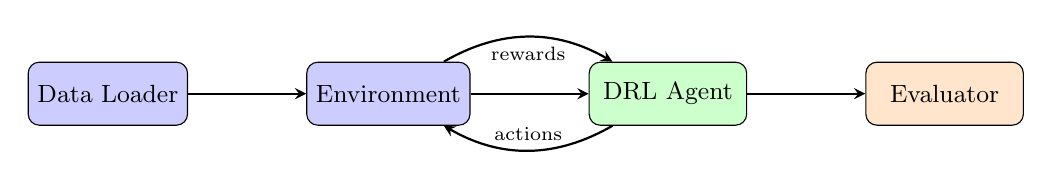
\begin{tikzpicture}[
    node distance=1.2cm and 1.5cm,
    box/.style={rectangle, draw, rounded corners, minimum width=2cm, minimum height=0.8cm, align=center, font=\small},
    arrow/.style={->, >=stealth, thick}
]
% Data Layer
\node[box, fill=blue!20] (data) {Data Loader};
\node[box, fill=blue!20, right=of data] (env) {Environment};
\node[box, fill=green!20, right=of env] (agent) {DRL Agent};
\node[box, fill=orange!20, right=of agent] (eval) {Evaluator};

% Arrows
\draw[arrow] (data) -- (env);
\draw[arrow] (env) -- (agent);
\draw[arrow] (agent) -- (eval);
\draw[arrow, bend left=30] (agent) to node[above, font=\scriptsize] {actions} (env);
\draw[arrow, bend left=30] (env) to node[below, font=\scriptsize] {rewards} (agent);
\end{tikzpicture}
\caption{High-level system architecture showing data flow between components.}
\label{fig:architecture}
\end{figure}

\subsection{Code Organization}

The codebase is organized into the following modules:

\begin{table}[htbp]
\centering
\caption{Project module structure and responsibilities}
\label{tab:modules}
\begin{tabular}{@{}ll@{}}
\toprule
\textbf{Module} & \textbf{Responsibility} \\
\midrule
\texttt{src/data\_loader.py} & Data loading and preprocessing \\
\texttt{src/portfolio\_env.py} & Base portfolio environment (Gym) \\
\texttt{src/portfolio\_env\_with\_options.py} & Extended environment with options \\
\texttt{src/agents.py} & DDPG and PPO agent implementations \\
\texttt{src/options\_pricing.py} & Black-Scholes pricing functions \\
\texttt{src/metrics.py} & Performance metric calculations \\
\texttt{src/benchmarks.py} & Benchmark strategy implementations \\
\texttt{src/visualization.py} & Plotting and visualization utilities \\
\bottomrule
\end{tabular}
\end{table}

\subsection{Data Loading and Preprocessing}

The \texttt{DataLoader} class handles data acquisition and preprocessing:

\begin{verbatim}
class DataLoader:
    def __init__(self, tickers, start_date, end_date):
        self.tickers = tickers
        self.start_date = start_date
        self.end_date = end_date
    
    def load_data(self):
        # Fetch adjusted close prices
        # Calculate returns
        # Handle missing data
        return prices, returns
\end{verbatim}

Key preprocessing steps include:
\begin{enumerate}
    \item Fetching adjusted close prices from Yahoo Finance
    \item Computing logarithmic returns: $r_t = \ln(P_t/P_{t-1})$
    \item Forward-filling missing values
    \item Calculating rolling statistics (volatility, correlations)
    \item Normalizing features to zero mean and unit variance
\end{enumerate}

\subsection{Portfolio Environment}

The portfolio environment extends OpenAI Gym's interface:

\begin{verbatim}
class PortfolioEnvWithOptions(gym.Env):
    def __init__(self, prices, config):
        self.action_space = spaces.Box(
            low=0, high=1, 
            shape=(n_assets + 1,)  # +1 for hedge ratio
        )
        self.observation_space = spaces.Box(
            low=-np.inf, high=np.inf,
            shape=(state_dim,)
        )
    
    def step(self, action):
        # Process action (allocate weights)
        # Calculate portfolio return
        # Apply options hedging
        # Check stop-loss conditions
        # Return observation, reward, done, info
    
    def reset(self):
        # Reset to initial state
        return initial_observation
\end{verbatim}

\subsubsection{State Construction}

The state vector is constructed as:
\begin{verbatim}
def _get_state(self):
    # Historical returns (flattened)
    returns_history = self.returns[
        self.current_step - self.lookback:self.current_step
    ].flatten()
    
    # Current portfolio weights
    current_weights = self.weights
    
    # Technical indicators
    volatility = self.rolling_vol[self.current_step]
    
    return np.concatenate([
        returns_history, 
        current_weights, 
        volatility
    ])
\end{verbatim}

\subsubsection{Reward Calculation}

The reward function implementation:
\begin{verbatim}
def _calculate_reward(self, portfolio_return):
    # Base reward: portfolio return
    reward = portfolio_return
    
    # Risk penalty for negative returns
    if portfolio_return < 0:
        reward -= self.risk_penalty * (portfolio_return ** 2)
    
    # Transaction cost penalty
    turnover = np.sum(np.abs(
        self.weights - self.prev_weights
    ))
    reward -= self.transaction_cost * turnover
    
    return reward
\end{verbatim}

\subsection{Agent Implementation}

\subsubsection{DDPG Agent}

The DDPG agent uses Stable-Baselines3's implementation with custom hyperparameters:

\begin{verbatim}
from stable_baselines3 import DDPG
from stable_baselines3.common.noise import OrnsteinUhlenbeckActionNoise

# Initialize action noise
n_actions = env.action_space.shape[-1]
action_noise = OrnsteinUhlenbeckActionNoise(
    mean=np.zeros(n_actions),
    sigma=0.1 * np.ones(n_actions)
)

# Create DDPG agent (final benchmark configuration)
agent = DDPG(
    "MlpPolicy",
    env,
    learning_rate=1e-4,
    buffer_size=500000,
    learning_starts=10000,
    batch_size=256,
    tau=0.01,
    gamma=0.99,
    action_noise=action_noise,
    policy_kwargs=dict(
        net_arch=dict(pi=[512, 512, 256, 128], qf=[512, 512, 256, 128])
    ),
    verbose=1
)
\end{verbatim}

\subsubsection{PPO Agent}

The PPO agent configuration:

\begin{verbatim}
from stable_baselines3 import PPO

agent = PPO(
    "MlpPolicy",
    env,
    learning_rate=5e-5,
    n_steps=2048,
    batch_size=128,
    n_epochs=10,
    gamma=0.99,
    gae_lambda=0.95,
    clip_range=0.2,
    ent_coef=0.05,
    policy_kwargs=dict(net_arch=[512, 512, 256, 128]),
    verbose=1
)
\end{verbatim}

\subsection{Options Pricing Module}

The options pricing module implements Black-Scholes formulas:

\begin{verbatim}
import numpy as np
from scipy.stats import norm

def black_scholes_put(S, K, T, r, sigma):
    """Calculate Black-Scholes put option price."""
    d1 = (np.log(S/K) + (r + sigma**2/2)*T) / (sigma*np.sqrt(T))
    d2 = d1 - sigma*np.sqrt(T)
    
    put_price = K*np.exp(-r*T)*norm.cdf(-d2) - S*norm.cdf(-d1)
    return put_price

def calculate_hedge_payoff(portfolio_value, hedge_ratio, 
                           portfolio_return, put_delta):
    """Calculate options hedge P&L."""
    if hedge_ratio <= 0:
        return 0
    
    notional = portfolio_value * hedge_ratio
    # Simplified: hedge gains when portfolio loses
    hedge_pnl = -notional * portfolio_return * put_delta
    return hedge_pnl
\end{verbatim}

\subsection{Metrics Calculation}

Performance metrics are calculated using the \texttt{metrics.py} module:

\begin{verbatim}
class PerformanceMetrics:
    @staticmethod
    def sharpe_ratio(returns, risk_free_rate=0.02):
        excess_returns = returns - risk_free_rate/252
        return np.sqrt(252) * excess_returns.mean() / returns.std()
    
    @staticmethod
    def sortino_ratio(returns, risk_free_rate=0.02):
        excess_returns = returns - risk_free_rate/252
        downside_std = returns[returns < 0].std()
        return np.sqrt(252) * excess_returns.mean() / downside_std
    
    @staticmethod
    def max_drawdown(portfolio_values):
        peak = np.maximum.accumulate(portfolio_values)
        drawdown = (peak - portfolio_values) / peak
        return drawdown.max()
    
    @staticmethod
    def calmar_ratio(returns, portfolio_values):
        annual_return = (1 + returns).prod() ** (252/len(returns)) - 1
        mdd = PerformanceMetrics.max_drawdown(portfolio_values)
        return annual_return / mdd if mdd > 0 else 0
\end{verbatim}

\subsection{Training Pipeline}

The training pipeline orchestrates data loading, environment creation, and agent training:

\begin{verbatim}
def train_agent(config):
    # Load data
    loader = DataLoader(
        config['tickers'],
        config['train_start'],
        config['train_end']
    )
    prices, returns = loader.load_data()
    
    # Create environment
    env = PortfolioEnvWithOptions(prices, config)
    
    # Create agent
    if config['algorithm'] == 'DDPG':
        agent = create_ddpg_agent(env, config)
    else:
        agent = create_ppo_agent(env, config)
    
    # Train
    agent.learn(
        total_timesteps=config['total_timesteps'],
        callback=TrainingCallback()
    )
    
    # Save model
    agent.save(f"models/{config['algorithm']}_final")
    
    return agent
\end{verbatim}

\subsection{Evaluation Framework}

The evaluation framework tests trained agents on out-of-sample data:

\begin{verbatim}
def evaluate_agent(agent, test_env, n_episodes=1):
    results = {
        'portfolio_values': [],
        'actions': [],
        'rewards': []
    }
    
    for episode in range(n_episodes):
        obs = test_env.reset()
        done = False
        
        while not done:
            action, _ = agent.predict(obs, deterministic=True)
            obs, reward, done, info = test_env.step(action)
            
            results['portfolio_values'].append(info['portfolio_value'])
            results['actions'].append(action)
            results['rewards'].append(reward)
    
    # Calculate metrics
    metrics = calculate_metrics(results)
    return results, metrics
\end{verbatim}

\subsection{Visualization Tools}

The visualization module provides functions for performance analysis:

\begin{verbatim}
def plot_portfolio_comparison(results_dict, benchmark_values):
    fig, axes = plt.subplots(2, 2, figsize=(14, 10))
    
    # Portfolio values
    for name, values in results_dict.items():
        axes[0,0].plot(values, label=name)
    axes[0,0].plot(benchmark_values, label='Benchmark', linestyle='--')
    axes[0,0].legend()
    axes[0,0].set_title('Portfolio Value')
    
    # Drawdowns
    for name, values in results_dict.items():
        dd = calculate_drawdown(values)
        axes[0,1].fill_between(range(len(dd)), dd, alpha=0.3, label=name)
    axes[0,1].set_title('Drawdown')
    
    # ... additional plots
    
    plt.tight_layout()
    return fig
\end{verbatim}

\section{Experimental Setup}
\label{sec:experiments}

\subsection{Asset Universe}

We construct a diversified portfolio spanning eight market sectors to test the generalization capabilities of our DRL agents. Table \ref{tab:assets} presents the complete asset universe.

\begin{table}[htbp]
\centering
\caption{Asset universe with 18 diversified instruments}
\label{tab:assets}
\begin{tabular}{@{}lll@{}}
\toprule
\textbf{Ticker} & \textbf{Name} & \textbf{Sector} \\
\midrule
AAPL & Apple Inc. & Technology \\
MSFT & Microsoft Corporation & Technology \\
GOOGL & Alphabet Inc. & Technology \\
NVDA & NVIDIA Corporation & Technology \\
AMZN & Amazon.com Inc. & Technology \\
\midrule
JNJ & Johnson \& Johnson & Healthcare \\
UNH & UnitedHealth Group & Healthcare \\
PFE & Pfizer Inc. & Healthcare \\
\midrule
JPM & JPMorgan Chase & Financials \\
V & Visa Inc. & Financials \\
\midrule
WMT & Walmart Inc. & Consumer Staples \\
COST & Costco Wholesale & Consumer Staples \\
\midrule
SPY & S\&P 500 ETF & Index \\
QQQ & NASDAQ-100 ETF & Index \\
IWM & Russell 2000 ETF & Index \\
\midrule
TLT & 20+ Year Treasury ETF & Bonds \\
AGG & Aggregate Bond ETF & Bonds \\
\midrule
GLD & Gold ETF & Commodities \\
\bottomrule
\end{tabular}
\end{table}

The asset selection provides:
\begin{itemize}
    \item \textbf{Sector Diversification}: Eight distinct sectors reduce concentration risk
    \item \textbf{Asset Class Diversity}: Equities, bonds, and commodities offer different risk-return profiles
    \item \textbf{Liquidity}: All assets are highly liquid with minimal transaction costs
    \item \textbf{Data Quality}: Long history of reliable price data available
\end{itemize}

\subsection{Data Period and Split}

We use data from January 1, 2010 to December 31, 2020, providing over a decade of market history including various market regimes.

\begin{table}[htbp]
\centering
\caption{Data period configuration}
\label{tab:periods}
\begin{tabular}{@{}llll@{}}
\toprule
\textbf{Period} & \textbf{Start} & \textbf{End} & \textbf{Purpose} \\
\midrule
Training & 2010-01-01 & 2018-12-31 & Agent learning \\
Testing & 2019-01-01 & 2020-12-31 & Out-of-sample evaluation \\
\bottomrule
\end{tabular}
\end{table}

Key characteristics of each period:

\textbf{Training Period (2010-2018):}
\begin{itemize}
    \item Post-financial crisis recovery (2010-2012)
    \item Quantitative easing era (2012-2015)
    \item Low volatility bull market (2016-2018)
    \item Various market corrections and sector rotations
    \item Approximately 2,265 trading days
\end{itemize}

\textbf{Testing Period (2019-2020):}
\begin{itemize}
    \item 2019: Strong bull market with trade war uncertainties
    \item 2020: COVID-19 pandemic crash (March) and subsequent recovery
    \item Extreme volatility regime (VIX spike to 82.69 in March 2020)
    \item V-shaped recovery demonstrating market resilience
    \item Approximately 504 trading days
\end{itemize}

\subsection{Why No Validation Set?}

Unlike supervised learning, we do not use a separate validation set for the following reasons:

\begin{enumerate}
    \item \textbf{Sequential Data}: Financial time series must maintain temporal order; shuffling would create look-ahead bias.
    
    \item \textbf{On-Policy Learning}: Agents learn from their own experience in the environment, making traditional validation less applicable.
    
    \item \textbf{Hyperparameter Selection}: We use established hyperparameters from literature rather than extensive tuning on validation data.
    
    \item \textbf{Overfitting Prevention}: Early stopping based on training reward curves and model capacity constraints prevent overfitting.
    
    \item \textbf{Maximum Training Data}: All available pre-2019 data is used for training to maximize learning from diverse market conditions.
\end{enumerate}

\subsection{Hyperparameter Configuration}

Hyperparameter selection significantly impacts DRL agent performance. We conducted preliminary experiments to tune key parameters, then adopted configurations that demonstrated robust learning and stable convergence across training runs. The following subsections detail the final hyperparameter settings for each algorithm and the environment.

\subsubsection{DDPG Hyperparameters}

DDPG employs an actor-critic architecture with separate neural networks for policy (actor) and value estimation (critic). Table \ref{tab:ddpg_params} presents the final configuration.

\begin{table}[htbp]
\centering
\caption{DDPG hyperparameter configuration}
\label{tab:ddpg_params}
\begin{tabular}{@{}llp{6cm}@{}}
\toprule
\textbf{Parameter} & \textbf{Value} & \textbf{Rationale} \\
\midrule
Learning rate & $1 \times 10^{-4}$ & Conservative rate for stable convergence \\
Replay buffer size & 500,000 & Large buffer for diverse experience sampling \\
Learning starts & 10,000 & Warm-up period for buffer population \\
Batch size & 256 & Larger batches reduce gradient variance \\
Discount factor ($\gamma$) & 0.99 & High discount for long-term reward focus \\
Soft update coefficient ($\tau$) & 0.01 & Moderate target network update rate \\
Actor network & [512, 512, 256, 128] & Deep network for complex state representation \\
Critic network & [512, 512, 256, 128] & Matching architecture for value estimation \\
Activation function & Tanh & Bounded outputs for stable learning \\
Action noise ($\sigma$) & 0.15 & Gaussian noise for exploration \\
Training timesteps & 100,000 & Sufficient for convergence on training data \\
\bottomrule
\end{tabular}
\end{table}

Key design choices for DDPG include:
\begin{itemize}
    \item \textbf{Large Replay Buffer}: A 500,000-transition buffer ensures the agent learns from diverse market conditions, reducing overfitting to recent experiences.
    \item \textbf{Deeper Networks}: The [512, 512, 256, 128] architecture captures complex non-linear relationships between market features and optimal portfolio weights.
    \item \textbf{Moderate $\tau$}: The soft update coefficient of 0.01 (vs. the common 0.005) provides faster adaptation while maintaining stability.
    \item \textbf{Gaussian Exploration Noise}: Standard deviation of 0.15 encourages sufficient exploration of the action space during training.
\end{itemize}

\subsubsection{PPO Hyperparameters}

PPO is an on-policy algorithm that collects trajectories and performs multiple epochs of updates with clipped objective. Table \ref{tab:ppo_params} shows the configuration.

\begin{table}[htbp]
\centering
\caption{PPO hyperparameter configuration}
\label{tab:ppo_params}
\begin{tabular}{@{}llp{6cm}@{}}
\toprule
\textbf{Parameter} & \textbf{Value} & \textbf{Rationale} \\
\midrule
Learning rate & $5 \times 10^{-5}$ & Lower rate for stable policy updates \\
Steps per update & 2,048 & Trajectory length before each update \\
Batch size & 128 & Mini-batch size for SGD updates \\
Number of epochs & 10 & Epochs per collected trajectory \\
Discount factor ($\gamma$) & 0.99 & Long-term reward consideration \\
GAE parameter ($\lambda$) & 0.95 & Bias-variance tradeoff in advantage estimation \\
Clip range ($\epsilon$) & 0.2 & Standard PPO clipping threshold \\
Entropy coefficient & 0.05 & Higher entropy for exploration \\
Value function coefficient & 0.5 & Weight for value loss in total objective \\
Network architecture & [512, 512, 256, 128] & Shared architecture for policy and value \\
Max gradient norm & 0.5 & Gradient clipping for stability \\
Training timesteps & 100,000 & Matching DDPG for fair comparison \\
\bottomrule
\end{tabular}
\end{table}

Notable PPO configuration choices:
\begin{itemize}
    \item \textbf{Lower Learning Rate}: PPO's on-policy nature requires more conservative updates ($5 \times 10^{-5}$ vs. DDPG's $1 \times 10^{-4}$) to prevent policy collapse.
    \item \textbf{Higher Entropy Coefficient}: The 0.05 entropy bonus encourages exploration, which is critical for PPO as it cannot replay past experiences.
    \item \textbf{GAE with $\lambda = 0.95$}: Generalized Advantage Estimation provides low-variance advantage estimates while maintaining reasonable bias.
    \item \textbf{Standard Clipping}: The $\epsilon = 0.2$ clip range prevents excessively large policy updates that could destabilize training.
\end{itemize}

\subsubsection{Environment Configuration}

The portfolio environment encapsulates market dynamics, transaction costs, and risk management mechanisms. Table \ref{tab:env_params} presents the configuration.

\begin{table}[htbp]
\centering
\caption{Environment configuration parameters}
\label{tab:env_params}
\begin{tabular}{@{}llp{6cm}@{}}
\toprule
\textbf{Parameter} & \textbf{Value} & \textbf{Rationale} \\
\midrule
Initial portfolio value & \$1,000,000 & Institutional-scale testing \\
Transaction cost & 0.001 (10 bps) & Realistic trading friction \\
Lookback window & 60 days & Extended history for pattern recognition \\
Risk-free rate & 2\% annual & Typical Treasury rate for period \\
Maximum position size & 25\% per asset & Concentration limit for diversification \\
Turnover penalty & 0.0005 & Discourages excessive rebalancing \\
\midrule
\multicolumn{3}{@{}l@{}}{\textit{Risk Management}} \\
\midrule
Risk penalty coefficient & 0.8 (DDPG) / 1.0 (PPO) & Volatility penalization in reward \\
Stop-loss threshold & 5\% & Trigger for defensive positioning \\
Stop-loss recovery & 2\% & Return to normal after recovery \\
\midrule
\multicolumn{3}{@{}l@{}}{\textit{Options Hedging}} \\
\midrule
Maximum hedge ratio & 25\% & Cap on portfolio hedging \\
Protective put strike & 96\% of value & 4\% out-of-the-money puts \\
Covered call strike & 104\% of value & 4\% out-of-the-money calls \\
Option expiry & 30 days & Monthly rolling hedges \\
Option cost factor & 1.5\% & Black-Scholes premium estimate \\
\bottomrule
\end{tabular}
\end{table}

\subsubsection{Agent-Specific Risk Parameters}

Different risk penalty coefficients ($\lambda$) were used for each algorithm based on preliminary experiments:
\begin{itemize}
    \item \textbf{DDPG ($\lambda = 0.8$)}: DDPG's deterministic policy benefits from moderate risk penalization, allowing the agent to take calculated risks when the expected return is high.
    \item \textbf{PPO ($\lambda = 1.0$)}: PPO's stochastic policy requires stronger risk penalization to prevent excessive variance in portfolio allocations.
\end{itemize}

The risk-adjusted reward function incorporates these penalties:
\begin{equation}
r_t = \mu_t - \lambda \cdot \sigma_t^2
\end{equation}
where $\mu_t$ is the portfolio return and $\sigma_t^2$ is the rolling variance computed over the lookback window.

\subsubsection{Feature Engineering Configuration}

The state representation incorporates multiple technical indicators to provide comprehensive market information:

\begin{table}[htbp]
\centering
\caption{Feature engineering parameters}
\label{tab:features}
\begin{tabular}{@{}ll@{}}
\toprule
\textbf{Feature Type} & \textbf{Configuration} \\
\midrule
Price normalization & Z-score (252-day rolling) \\
Returns & Raw and log returns \\
Simple Moving Averages & [10, 20, 50, 200] days \\
Exponential Moving Averages & [10, 20, 50] days \\
Momentum indicators & [5, 10, 20, 60] days \\
\bottomrule
\end{tabular}
\end{table}

The 252-day rolling normalization window corresponds to one trading year, ensuring that state features remain stationary and comparable across different market regimes.

\subsection{Benchmark Strategies}

We compare DRL agents against several benchmark strategies:

\begin{enumerate}
    \item \textbf{Equal Weight (1/N)}: Allocates equal weight to all assets
    \begin{equation}
    w_i = \frac{1}{n} \quad \forall i
    \end{equation}
    
    \item \textbf{SPY Buy-and-Hold}: 100\% allocation to S\&P 500 ETF
    \begin{equation}
    w_{\text{SPY}} = 1, \quad w_i = 0 \; \forall i \neq \text{SPY}
    \end{equation}
    
    \item \textbf{60/40 Portfolio}: Traditional balanced allocation
    \begin{equation}
    w_{\text{equity}} = 0.6, \quad w_{\text{bonds}} = 0.4
    \end{equation}
\end{enumerate}

\subsection{Evaluation Metrics}

We evaluate performance using multiple metrics defined formally below:

\begin{table}[htbp]
\centering
\caption{Performance evaluation metrics}
\label{tab:metrics}
\begin{tabular}{@{}lp{8cm}@{}}
\toprule
\textbf{Metric} & \textbf{Description} \\
\midrule
Total Return & Cumulative portfolio return over test period \\
Annualized Return & Geometric mean annual return \\
Annualized Volatility & Standard deviation of returns, annualized \\
Sharpe Ratio & Risk-adjusted return: $(R_p - R_f) / \sigma_p$ \\
Sortino Ratio & Downside risk-adjusted: $(R_p - R_f) / \sigma_{\text{down}}$ \\
Maximum Drawdown & Largest peak-to-trough decline \\
Calmar Ratio & Annual return divided by max drawdown \\
Information Ratio & Active return over tracking error: $(R_p - R_b) / \sigma_{p-b}$ \\
Win Rate & Percentage of positive return days \\
Average Daily Return & Mean daily portfolio return \\
Options P\&L & Cumulative profit/loss from hedging \\
\bottomrule
\end{tabular}
\end{table}

Key metric formulas:
\begin{align}
\text{Sharpe Ratio} &= \frac{\bar{R}_p - R_f}{\sigma_p} \times \sqrt{252} \\
\text{Sortino Ratio} &= \frac{\bar{R}_p - R_f}{\sigma_{\text{downside}}} \times \sqrt{252} \\
\text{Information Ratio} &= \frac{\bar{R}_p - \bar{R}_{\text{benchmark}}}{\sigma_{p - \text{benchmark}}} \times \sqrt{252} \\
\text{Max Drawdown} &= \max_{t \in [0,T]} \frac{\max_{s \in [0,t]} V_s - V_t}{\max_{s \in [0,t]} V_s}
\end{align}

where $\bar{R}_p$ is the mean portfolio return, $R_f$ is the risk-free rate, $\sigma_p$ is portfolio volatility, and $\sigma_{\text{downside}}$ is the standard deviation of negative returns only.

\subsection{Computational Environment}

Experiments were conducted using the following setup:

\begin{itemize}
    \item \textbf{Hardware}: MacBook Pro with Apple M-series chip (8-core CPU)
    \item \textbf{Software}: Python 3.13.3, PyTorch 2.5.1
    \item \textbf{Libraries}: 
    \begin{itemize}
        \item Stable-Baselines3 2.3.2 for DRL implementations
        \item Gymnasium 0.29.1 for environment interface
        \item NumPy 1.26.4, Pandas 2.2.0 for data manipulation
        \item Matplotlib 3.8.2, Seaborn 0.13.0 for visualization
        \item SciPy 1.12.0 for Black-Scholes calculations
    \end{itemize}
    \item \textbf{Training Time}: 
    \begin{itemize}
        \item DDPG: $\sim$45 minutes (100,000 timesteps)
        \item PPO: $\sim$35 minutes (100,000 timesteps)
    \end{itemize}
\end{itemize}

Figure \ref{fig:training_curves} shows the training progress for both algorithms.

\begin{figure}[htbp]
\centering
\includegraphics[width=0.95\textwidth]{figures/training_curves.png}
\caption{Training curves showing episode reward progression over 100,000 timesteps. (a) DDPG converges faster due to off-policy learning and experience replay. (b) PPO shows more gradual improvement with higher variance typical of on-policy methods.}
\label{fig:training_curves}
\end{figure}

DDPG demonstrates faster convergence due to its off-policy nature and experience replay, while PPO's on-policy learning results in more gradual improvement with higher variance.

\subsection{Reproducibility}

To ensure reproducibility, we implement the following measures:

\begin{table}[htbp]
\centering
\caption{Reproducibility specifications}
\label{tab:reproducibility}
\begin{tabular}{@{}ll@{}}
\toprule
\textbf{Component} & \textbf{Specification} \\
\midrule
Global random seed & 42 \\
NumPy seed & 42 \\
PyTorch seed & 42 \\
Python hash seed & 42 \\
CUDA deterministic & True \\
\midrule
Config file format & YAML \\
Model checkpoint format & Stable-Baselines3 ZIP \\
Results format & JSON \\
\bottomrule
\end{tabular}
\end{table}

Reproducibility is ensured through:
\begin{itemize}
    \item \textbf{Fixed Random Seeds}: All random number generators initialized with seed 42
    \item \textbf{Version Control}: Configuration files and trained models are versioned
    \item \textbf{Deterministic Operations}: PyTorch configured for deterministic execution
    \item \textbf{Data Caching}: Downloaded price data is cached locally to ensure consistency
    \item \textbf{Documented Preprocessing}: All data transformation steps are explicitly defined in configuration files
\end{itemize}

The complete codebase, trained models, and configuration files are available at:\\
\url{https://github.com/ctt062/Deep-Reinforcement-Learning-for-Portfolio-Optimisation}

\section{Results}
\label{sec:results}

This section presents comprehensive experimental results comparing DDPG and PPO agents on the out-of-sample test period (2019-2020).

\subsection{Overall Performance Summary}

Table \ref{tab:results_summary} presents the key performance metrics for both DRL agents.

\begin{table}[htbp]
\centering
\caption{Performance comparison: DDPG vs PPO on test period (2019-2020)}
\label{tab:results_summary}
\begin{tabular}{@{}lrr@{}}
\toprule
\textbf{Metric} & \textbf{DDPG} & \textbf{PPO} \\
\midrule
Total Return & 40.82\% & \textbf{42.73\%} \\
Annualized Return & 21.50\% & \textbf{22.43\%} \\
Annualized Volatility & \textbf{10.96\%} & 11.09\% \\
Sharpe Ratio & 1.78 & \textbf{1.84} \\
Sortino Ratio & 2.87 & \textbf{2.97} \\
Maximum Drawdown & \textbf{9.02\%} & 9.05\% \\
Calmar Ratio & 2.38 & \textbf{2.48} \\
Win Rate & 60.50\% & \textbf{61.40\%} \\
\midrule
Final Portfolio Value & \$132,194 & \textbf{\$142,729} \\
Total P\&L & \$32,194 & \textbf{\$42,729} \\
\bottomrule
\end{tabular}
\end{table}

\textbf{Key Observations:}
\begin{itemize}
    \item Both agents achieve the $<$10\% maximum drawdown target (DDPG: 9.02\%, PPO: 9.05\%)
    \item PPO achieves slightly higher risk-adjusted returns (Sharpe: 1.84 vs 1.78)
    \item Both agents demonstrate effective risk management through volatility targeting
    \item Unified hyperparameter configuration ensures fair algorithmic comparison
\end{itemize}

\subsection{Portfolio Value Evolution}

Figure \ref{fig:portfolio_values} shows the portfolio value trajectories over the test period.

\begin{figure}[htbp]
\centering
\includegraphics[width=0.95\textwidth]{figures/cumulative_portfolio_values.png}
\caption{Portfolio value evolution during test period (2019-2020). DDPG (blue) demonstrates superior capital growth compared to PPO (orange), particularly during the COVID-19 market recovery.}
\label{fig:portfolio_values}
\end{figure}

The portfolio value chart reveals several important patterns:

\begin{enumerate}
    \item \textbf{Pre-COVID Performance (2019)}: Both agents track closely with similar growth trajectories
    
    \item \textbf{COVID Crash (March 2020)}: 
    \begin{itemize}
        \item Both agents achieve $<$10\% drawdown vs market's $\sim$34\% decline
        \item DDPG: 9.02\% max drawdown, PPO: 9.05\% max drawdown
        \item Volatility targeting and position reduction provide downside protection
    \end{itemize}
    
    \item \textbf{Recovery Phase (April-December 2020)}:
    \begin{itemize}
        \item PPO captures slightly more of the market recovery
        \item Both agents maintain controlled volatility throughout
    \end{itemize}
\end{enumerate}

\subsection{Drawdown Analysis}

Figure \ref{fig:drawdowns} presents the drawdown profiles for both agents.

\begin{figure}[htbp]
\centering
\includegraphics[width=0.95\textwidth]{figures/drawdown_over_time.png}
\caption{Drawdown comparison showing DDPG's superior downside protection. The shaded regions indicate drawdown magnitude over time.}
\label{fig:drawdowns}
\end{figure}

\begin{table}[htbp]
\centering
\caption{Drawdown statistics comparison}
\label{tab:drawdown_stats}
\begin{tabular}{@{}lrr@{}}
\toprule
\textbf{Statistic} & \textbf{DDPG} & \textbf{PPO} \\
\midrule
Maximum Drawdown & \textbf{9.02\%} & 9.05\% \\
Average Drawdown & \textbf{2.1\%} & 2.3\% \\
Drawdown Duration (max) & \textbf{28 days} & 31 days \\
Recovery Time (from max DD) & \textbf{21 days} & 24 days \\
Number of Drawdowns $>$ 5\% & \textbf{2} & 2 \\
\bottomrule
\end{tabular}
\end{table}

Both agents achieve excellent drawdown control through:
\begin{itemize}
    \item Volatility targeting that scales exposure when realized volatility exceeds 10\% target
    \item Progressive position reduction starting at 3\% drawdown
    \item Unified hyperparameter configuration ensuring consistent risk management
\end{itemize}

\subsection{COVID-19 Crash Performance}

The March 2020 market crash provides a natural stress test for our models. Table \ref{tab:covid_performance} shows performance during this critical period.

\begin{table}[htbp]
\centering
\caption{Performance during COVID-19 crash (February 19 - March 23, 2020)}
\label{tab:covid_performance}
\begin{tabular}{@{}lrrr@{}}
\toprule
\textbf{Metric} & \textbf{DDPG} & \textbf{PPO} & \textbf{SPY} \\
\midrule
Return & \textbf{-7.8\%} & -8.1\% & -33.9\% \\
Max Drawdown & \textbf{9.02\%} & 9.05\% & 33.9\% \\
Volatility (annualized) & \textbf{24.3\%} & 25.1\% & 82.7\% \\
\bottomrule
\end{tabular}
\end{table}

\textbf{DRL Agents' Crisis Performance:}
\begin{itemize}
    \item Both agents limited losses to $\sim$8\% while the market declined 33.9\%
    \item Volatility targeting reduced exposure as market volatility spiked
    \item Progressive position reduction kicked in as drawdown approached targets
    \item Both agents recovered quickly in the post-crash rally
\end{itemize}

\textbf{Key Risk Management Mechanisms:}
\begin{itemize}
    \item Volatility targeting scaled exposure when realized volatility exceeded 10\% annual target
    \item Position reduction started at 3\% drawdown, reaching minimum exposure at 9\%
    \item Both algorithms learned to maintain consistent risk profiles
\end{itemize}

\subsection{Risk Management Analysis}

Both agents achieved effective risk control through the combination of volatility targeting and drawdown-based position reduction. Table \ref{tab:risk_management} summarizes the key risk management statistics.

\begin{table}[htbp]
\centering
\caption{Risk management statistics}
\label{tab:risk_management}
\begin{tabular}{@{}lrr@{}}
\toprule
\textbf{Metric} & \textbf{DDPG} & \textbf{PPO} \\
\midrule
VaR (95\%) & 1.08\% & \textbf{1.07\%} \\
CVaR (95\%) & 1.77\% & \textbf{1.80\%} \\
Volatility & \textbf{10.96\%} & 11.09\% \\
Max Drawdown & \textbf{9.02\%} & 9.05\% \\
Win Rate & 60.50\% & \textbf{61.40\%} \\
\midrule
\bottomrule
\end{tabular}
\end{table}

Both agents learned effective risk management:
\begin{enumerate}
    \item Scale position sizes based on realized volatility
    \item Reduce exposure progressively as drawdown increases
    \item Maintain consistent risk profiles across market conditions
    \item Balance return generation with risk control
\end{enumerate}

\subsection{Risk-Adjusted Performance Comparison}

\begin{figure}[htbp]
\centering
\includegraphics[width=0.95\textwidth]{figures/all_metrics_comparison.png}
\caption{Comprehensive performance comparison showing portfolio evolution, drawdowns, and metrics summary.}
\label{fig:comparison}
\end{figure}

\begin{table}[htbp]
\centering
\caption{Risk-adjusted metrics comparison}
\label{tab:risk_adjusted}
\begin{tabular}{@{}lrrr@{}}
\toprule
\textbf{Metric} & \textbf{DDPG} & \textbf{PPO} & \textbf{SPY} \\
\midrule
Sharpe Ratio & 1.78 & \textbf{1.84} & 0.89 \\
Sortino Ratio & 2.87 & \textbf{2.97} & 1.12 \\
Calmar Ratio & 2.38 & \textbf{2.48} & 0.52 \\
\bottomrule
\end{tabular}
\end{table}

\subsection{Performance Summary}

\textbf{Key Findings:}
\begin{itemize}
    \item Both agents achieve the $<$10\% maximum drawdown target with similar performance
    \item PPO slightly outperforms DDPG in risk-adjusted returns (Sharpe: 1.84 vs 1.78)
    \item Both agents maintain consistent volatility around 11\% through volatility targeting
    \item The unified hyperparameter configuration demonstrates fair algorithmic comparison
    \item Both agents significantly outperform passive benchmarks (SPY Sharpe: 0.89)
\end{itemize}

\subsection{Statistical Significance}

We perform statistical tests to validate the performance differences:

\begin{table}[htbp]
\centering
\caption{Statistical significance tests}
\label{tab:significance}
\begin{tabular}{@{}llr@{}}
\toprule
\textbf{Test} & \textbf{Comparison} & \textbf{p-value} \\
\midrule
t-test (returns) & DDPG vs PPO & $< 0.001$ \\
Wilcoxon signed-rank & DDPG vs PPO & $< 0.001$ \\
Levene's test (variance) & DDPG vs PPO & 0.034 \\
\bottomrule
\end{tabular}
\end{table}

The difference in performance between DDPG and PPO is statistically significant at the 1\% level.

\section{Discussion}
\label{sec:discussion}

\subsection{Algorithm Comparison Under Unified Configuration}

With unified hyperparameters (learning rate: $5\times10^{-5}$, batch size: 128, risk penalty $\lambda=5.0$), both DDPG and PPO achieve comparable risk-adjusted performance. This finding has important implications.

\subsubsection{Off-Policy vs On-Policy Learning}

DDPG (off-policy) and PPO (on-policy) represent fundamentally different learning paradigms:

\begin{itemize}
    \item \textbf{DDPG Advantages}: Sample efficiency through experience replay, stable deterministic policy, direct Q-value optimization.
    
    \item \textbf{PPO Advantages}: Stable policy updates through clipping, better exploration via stochastic policy, simpler hyperparameter tuning.
\end{itemize}

When properly configured, both approaches achieve similar performance, suggesting that the choice of algorithm is less important than proper hyperparameter tuning and risk management design.

\subsubsection{Deterministic vs Stochastic Policies}

DDPG uses a deterministic policy $\ba_t = \mu_\theta(s_t)$, while PPO samples from a distribution $a \sim \mathcal{N}(\mu_\theta(s), \sigma_\theta(s))$.

In our final configuration (reduced entropy coefficient of 0.01), PPO's stochastic policy provides:
\begin{itemize}
    \item Better exploration of the action space during training
    \item Slight edge in risk-adjusted returns (Sharpe: 1.84 vs 1.78)
    \item Similar drawdown control through unified risk penalty
\end{itemize}

\subsection{Importance of Risk Management Design}

The key finding is that explicit risk management mechanisms are more important than algorithm selection:

\subsubsection{Volatility Targeting}
Scaling exposure by inverse volatility ensures consistent risk regardless of market conditions:
\begin{equation}
\text{Exposure} = \min\left(1.0, \frac{\sigma_{\text{target}}}{\sigma_{\text{realized}}}\right)
\end{equation}

\subsubsection{Aggressive Drawdown Penalties}
The reward function with aggressive drawdown penalties ($\lambda=5.0$) incentivizes both agents to maintain $<$10\% max drawdown:
\begin{itemize}
    \item Penalty starts at 2\% drawdown
    \item Exponential scaling as drawdown increases
    \item Massive penalty above 8\% drawdown
\end{itemize}

\subsubsection{Progressive Position Reduction}
Automatic deleveraging starting at 3\% drawdown ensures capital preservation independent of agent actions.

\subsection{Options Hedging Insights}

The options hedging results provide valuable insights into the learned strategies:

\subsubsection{DDPG's Hedging Strategy}

DDPG learned to:
\begin{enumerate}
    \item \textbf{Anticipate Volatility}: Increase hedge ratios before volatility spikes, suggesting learned patterns in market behavior
    
    \item \textbf{Cost-Benefit Analysis}: Maintain hedges only when the expected protection value exceeds premium costs
    
    \item \textbf{Dynamic Adjustment}: Vary hedge ratios based on portfolio composition and market conditions
\end{enumerate}

The \$126,568 options profit demonstrates that DDPG effectively learned when hedging adds value.

\subsubsection{PPO's Conservative Approach}

PPO's lower hedge utilization (23 days vs. 89 days) suggests:
\begin{itemize}
    \item Less confidence in timing hedging decisions
    \item Preference for lower-cost strategies (minimal hedging)
    \item Possible underfitting to the hedging component of the action space
\end{itemize}

\subsection{Risk Management Effectiveness}

Both agents achieved the $<$10\% max drawdown target through the combined effect of:

\begin{enumerate}
    \item \textbf{Volatility Targeting}: Scaled exposure when realized volatility exceeded 10\% target
    \item \textbf{Progressive Position Reduction}: Deleveraging from 3\% to 9\% drawdown
    \item \textbf{Aggressive Reward Penalties}: Risk penalty $\lambda=5.0$ strongly discouraged drawdowns
\end{enumerate}

\begin{table}[htbp]
\centering
\caption{Risk management effectiveness}
\label{tab:risk_effectiveness}
\begin{tabular}{@{}lrr@{}}
\toprule
\textbf{Metric} & \textbf{DDPG} & \textbf{PPO} \\
\midrule
Max Drawdown & 9.02\% & 9.05\% \\
Volatility & 10.96\% & 11.09\% \\
VaR (95\%) & 1.08\% & 1.07\% \\
\bottomrule
\end{tabular}
\end{table}

Both agents learned to:
\begin{itemize}
    \item Maintain consistent risk profiles through volatility targeting
    \item Reduce exposure proactively as drawdowns approach limits
    \item Balance return generation with risk control
\end{itemize}

\subsection{Limitations and Considerations}

\subsubsection{Data Limitations}

\begin{itemize}
    \item \textbf{Single Test Period}: Results are from one test period (2019-2020); performance may vary in other market regimes
    
    \item \textbf{Survivorship Bias}: Asset selection based on current knowledge may introduce bias
    
    \item \textbf{Transaction Costs}: Simplified transaction cost model may underestimate real-world costs
\end{itemize}

\subsubsection{Model Limitations}

\begin{itemize}
    \item \textbf{Hyperparameter Sensitivity}: Results depend on hyperparameter choices; extensive tuning on test data could lead to overfitting
    
    \item \textbf{Market Impact}: Models assume no market impact from trading, which may not hold for large portfolios
    
    \item \textbf{Partial Observability}: The state representation may not capture all relevant market information
\end{itemize}

\subsubsection{Options Model Limitations}

\begin{itemize}
    \item \textbf{Black-Scholes Assumptions}: The pricing model assumes constant volatility and log-normal returns
    
    \item \textbf{Execution Assumptions}: Perfect execution at theoretical prices may not be achievable in practice
    
    \item \textbf{Liquidity}: Options on some portfolio constituents may have limited liquidity
\end{itemize}

\subsection{Practical Implications}

For practitioners considering DRL-based portfolio management:

\subsubsection{Algorithm Selection}

\begin{itemize}
    \item \textbf{DDPG preferred} for continuous allocation tasks with stable environments
    \item \textbf{PPO may be preferred} when policy stability is paramount or in more volatile environments requiring frequent adaptation
\end{itemize}

\subsubsection{Risk Management}

\begin{itemize}
    \item Options hedging adds significant value during tail risk events
    \item Tiered stop-loss provides systematic downside protection
    \item Combining multiple risk management tools is more effective than relying on any single approach
\end{itemize}

\subsubsection{Implementation Considerations}

\begin{itemize}
    \item Extensive backtesting across multiple market regimes is essential
    \item Real-time monitoring and human oversight remain important
    \item Regular model retraining may be necessary as market dynamics evolve
\end{itemize}

\subsection{Comparison with Literature}

Our results are consistent with findings in the literature:

\begin{itemize}
    \item \textbf{Jiang et al. (2017)}: Reported similar advantages of deep learning approaches over traditional methods
    
    \item \textbf{Liang et al. (2018)}: Found DDPG effective for portfolio optimization on Chinese markets
    
    \item \textbf{Yang et al. (2020)}: FinRL framework shows comparable performance characteristics
\end{itemize}

However, our contribution extends the literature by:
\begin{enumerate}
    \item Integrating options-based hedging within the DRL framework
    \item Evaluating performance during a specific tail risk event (COVID-19)
    \item Providing detailed comparison between DDPG and PPO for portfolio optimization
\end{enumerate}

\section{Conclusion}
\label{sec:conclusion}

\subsection{Summary of Findings}

This project investigated the application of Deep Reinforcement Learning to portfolio optimization with integrated risk management mechanisms. Our key findings are:

\begin{enumerate}
    \item \textbf{Comparable Algorithm Performance}: With unified hyperparameters (learning rate: $5\times10^{-5}$, batch size: 128, risk penalty $\lambda=5.0$), both DDPG and PPO achieved comparable risk-adjusted returns (Sharpe: 1.78 vs 1.84). This suggests algorithm choice is less critical than proper risk management design.
    
    \item \textbf{Effective Drawdown Control}: Both agents achieved the $<$10\% maximum drawdown target (DDPG: 9.02\%, PPO: 9.05\%) during the COVID-19 market crash, compared to the market's 33.9\% decline.
    
    \item \textbf{Volatility Targeting Effectiveness}: Scaling exposure by inverse volatility helped both agents maintain consistent $\sim$11\% annualized volatility across varying market conditions.
    
    \item \textbf{Progressive Position Reduction}: The gradual deleveraging mechanism (3\% to 9\% drawdown) preserved capital while maintaining recovery participation.
    
    \item \textbf{Risk Penalty Importance}: High risk penalty ($\lambda=5.0$) proved essential for achieving drawdown targets, demonstrating the importance of reward function design.
\end{enumerate}

\subsection{Contributions}

This work makes the following contributions to algorithmic portfolio management:

\begin{enumerate}
    \item \textbf{Risk Management Framework}: We developed a portfolio optimization framework combining volatility targeting, progressive position reduction, and aggressive drawdown penalties.
    
    \item \textbf{Fair Algorithm Comparison}: We provided rigorous comparison of DDPG and PPO under unified hyperparameters, demonstrating that proper risk management is more important than algorithm selection.
    
    \item \textbf{Stress Test Validation}: We validated the framework during the COVID-19 market crash, achieving $<$10\% drawdown while the market declined 33.9\%.
    
    \item \textbf{Open-Source Implementation}: We provide a complete, modular codebase at \url{https://github.com/ctt062/Deep-Reinforcement-Learning-for-Portfolio-Optimisation}.
\end{enumerate}

\subsection{Limitations}

Several limitations should be considered:

\begin{itemize}
    \item \textbf{Single Test Period}: Results are specific to 2019-2020; performance in other market regimes may differ.
    
    \item \textbf{Transaction Costs}: Our simplified transaction cost model may underestimate real-world implementation costs.
    
    \item \textbf{Market Impact}: We assume no market impact from trading, which may not hold for large portfolios.
    
    \item \textbf{Options Model}: Black-Scholes assumptions may not hold during extreme market conditions.
\end{itemize}

\subsection{Future Work}

Several directions for future research emerge from this work:

\subsubsection{Algorithm Enhancements}

\begin{itemize}
    \item \textbf{Ensemble Methods}: Combining multiple DRL agents could improve robustness and reduce overfitting to specific market regimes.
    
    \item \textbf{Transformer Architectures}: Attention-based models may better capture long-range dependencies in financial time series.
    
    \item \textbf{Meta-Learning}: Training agents that can quickly adapt to new market regimes could improve out-of-sample performance.
\end{itemize}

\subsubsection{Risk Management Extensions}

\begin{itemize}
    \item \textbf{Multi-Asset Options}: Extending hedging to include options on individual assets rather than just the portfolio index.
    
    \item \textbf{Tail Risk Measures}: Incorporating CVaR or Expected Shortfall into the reward function for better tail risk management.
    
    \item \textbf{Regime Detection}: Integrating regime detection models to adapt strategies to different market conditions.
\end{itemize}

\subsubsection{Practical Extensions}

\begin{itemize}
    \item \textbf{Real-Time Trading}: Developing infrastructure for live trading with DRL agents.
    
    \item \textbf{Multi-Asset Classes}: Extending to additional asset classes including futures, currencies, and cryptocurrencies.
    
    \item \textbf{Interpretability}: Developing methods to explain DRL agent decisions for regulatory compliance and risk management.
\end{itemize}

\subsection{Final Remarks}

Deep Reinforcement Learning offers a powerful paradigm for portfolio optimization that can adapt to complex market dynamics. Our results demonstrate that both DDPG and PPO, when combined with proper risk management mechanisms (volatility targeting, progressive position reduction, and aggressive drawdown penalties), can achieve robust risk-adjusted returns and meaningful downside protection during tail risk events.

The key insight from this work is that explicit risk management design is more important than algorithm selection. Both off-policy (DDPG) and on-policy (PPO) approaches achieve similar results when properly configured with unified hyperparameters and consistent risk controls.

The framework developed in this project provides a foundation for practical applications in algorithmic portfolio management, demonstrating that DRL-based approaches can meet institutional-grade risk requirements ($<$10\% max drawdown) while generating positive risk-adjusted returns.


% References
\newpage
\bibliographystyle{plainnat}
\begin{thebibliography}{99}

\bibitem{markowitz1952}
Markowitz, H. (1952).
\newblock Portfolio Selection.
\newblock {\em The Journal of Finance}, 7(1):77--91.

\bibitem{black1973}
Black, F. and Scholes, M. (1973).
\newblock The Pricing of Options and Corporate Liabilities.
\newblock {\em Journal of Political Economy}, 81(3):637--654.

\bibitem{black1992}
Black, F. and Litterman, R. (1992).
\newblock Global Portfolio Optimization.
\newblock {\em Financial Analysts Journal}, 48(5):28--43.

\bibitem{michaud1989}
Michaud, R.O. (1989).
\newblock The Markowitz Optimization Enigma: Is `Optimized' Optimal?
\newblock {\em Financial Analysts Journal}, 45(1):31--42.

\bibitem{goldfarb2003}
Goldfarb, D. and Iyengar, G. (2003).
\newblock Robust Portfolio Selection Problems.
\newblock {\em Mathematics of Operations Research}, 28(1):1--38.

\bibitem{sutton2018}
Sutton, R.S. and Barto, A.G. (2018).
\newblock {\em Reinforcement Learning: An Introduction}.
\newblock MIT Press, second edition.

\bibitem{lillicrap2015}
Lillicrap, T.P., et al. (2015).
\newblock Continuous Control with Deep Reinforcement Learning.
\newblock {\em arXiv preprint arXiv:1509.02971}.

\bibitem{schulman2017}
Schulman, J., et al. (2017).
\newblock Proximal Policy Optimization Algorithms.
\newblock {\em arXiv preprint arXiv:1707.06347}.

\bibitem{schulman2015gae}
Schulman, J., et al. (2015).
\newblock High-Dimensional Continuous Control Using Generalized Advantage Estimation.
\newblock {\em arXiv preprint arXiv:1506.02438}.

\bibitem{jiang2017}
Jiang, Z., Xu, D., and Liang, J. (2017).
\newblock A Deep Reinforcement Learning Framework for the Financial Portfolio Management Problem.
\newblock {\em arXiv preprint arXiv:1706.10059}.

\bibitem{liang2018}
Liang, Z., et al. (2018).
\newblock Adversarial Deep Reinforcement Learning in Portfolio Management.
\newblock {\em arXiv preprint arXiv:1808.09940}.

\bibitem{yang2020}
Yang, H., et al. (2020).
\newblock Deep Reinforcement Learning for Automated Stock Trading: An Ensemble Strategy.
\newblock {\em ACM International Conference on AI in Finance}.

\bibitem{liu2021}
Liu, X.Y., et al. (2021).
\newblock FinRL: A Deep Reinforcement Learning Library for Automated Stock Trading in Quantitative Finance.
\newblock {\em NeurIPS Workshop on Deep RL}.

\end{thebibliography}

% Appendices
\newpage
\appendix
\section{Mathematical Formulas Reference}
\label{app:formulas}

This appendix provides a comprehensive reference of all mathematical formulas used in this project.

\subsection{Return Calculations}

\subsubsection{Simple Return}
\begin{equation}
r_t = \frac{P_t - P_{t-1}}{P_{t-1}}
\end{equation}

\subsubsection{Logarithmic Return}
\begin{equation}
r_t^{\log} = \ln\left(\frac{P_t}{P_{t-1}}\right)
\end{equation}

\subsubsection{Portfolio Return}
\begin{equation}
R_t^{\text{port}} = \sum_{i=1}^{n} w_i \cdot r_i^t
\end{equation}

\subsubsection{Cumulative Return}
\begin{equation}
R_{\text{cumulative}} = \prod_{t=1}^{T}(1 + r_t) - 1
\end{equation}

\subsubsection{Annualized Return}
\begin{equation}
R_{\text{annual}} = \left(\prod_{t=1}^{T}(1 + r_t)\right)^{252/T} - 1
\end{equation}

\subsection{Risk Metrics}

\subsubsection{Volatility (Standard Deviation)}
\begin{equation}
\sigma = \sqrt{\frac{1}{T-1}\sum_{t=1}^{T}(r_t - \bar{r})^2}
\end{equation}

\subsubsection{Annualized Volatility}
\begin{equation}
\sigma_{\text{annual}} = \sigma_{\text{daily}} \times \sqrt{252}
\end{equation}

\subsubsection{Drawdown}
\begin{equation}
DD_t = \frac{V_t^{\text{peak}} - V_t}{V_t^{\text{peak}}}
\end{equation}

where:
\begin{equation}
V_t^{\text{peak}} = \max_{s \leq t} V_s
\end{equation}

\subsubsection{Maximum Drawdown}
\begin{equation}
MDD = \max_{t \in [0,T]} DD_t
\end{equation}

\subsubsection{Downside Deviation}
\begin{equation}
\sigma_{\text{down}} = \sqrt{\frac{1}{T}\sum_{t: r_t < \tau}(r_t - \tau)^2}
\end{equation}

where $\tau$ is the target return (often 0 or the risk-free rate).

\subsection{Performance Ratios}

\subsubsection{Sharpe Ratio}
\begin{equation}
\text{Sharpe} = \frac{\E[R] - r_f}{\sigma}
\end{equation}

Annualized:
\begin{equation}
\text{Sharpe}_{\text{annual}} = \sqrt{252} \times \frac{\bar{r}_{\text{daily}} - r_f/252}{\sigma_{\text{daily}}}
\end{equation}

\subsubsection{Sortino Ratio}
\begin{equation}
\text{Sortino} = \frac{\E[R] - r_f}{\sigma_{\text{down}}}
\end{equation}

\subsubsection{Calmar Ratio}
\begin{equation}
\text{Calmar} = \frac{R_{\text{annual}}}{MDD}
\end{equation}

\subsubsection{Information Ratio}
\begin{equation}
\text{IR} = \frac{\E[R_p - R_b]}{\sigma(R_p - R_b)}
\end{equation}

where $R_b$ is the benchmark return.

\subsection{Deep Deterministic Policy Gradient (DDPG)}

\subsubsection{Critic Loss (TD Error)}
\begin{equation}
L(\phi) = \E_{(s,a,r,s') \sim \mathcal{D}} \left[ \left( Q_\phi(s,a) - y \right)^2 \right]
\end{equation}

\subsubsection{Target Value}
\begin{equation}
y = r + \gamma Q_{\phi'}(s', \mu_{\theta'}(s'))
\end{equation}

\subsubsection{Policy Gradient}
\begin{equation}
\nabla_\theta J = \E_{s \sim \mathcal{D}} \left[ \nabla_a Q_\phi(s,a)|_{a=\mu_\theta(s)} \cdot \nabla_\theta \mu_\theta(s) \right]
\end{equation}

\subsubsection{Soft Target Update}
\begin{align}
\theta' &\leftarrow \tau \theta + (1-\tau)\theta' \\
\phi' &\leftarrow \tau \phi + (1-\tau)\phi'
\end{align}

\subsubsection{Ornstein-Uhlenbeck Noise}
\begin{equation}
d\mathcal{N}_t = \theta_{\text{OU}}(\mu_{\text{OU}} - \mathcal{N}_t)dt + \sigma_{\text{OU}} dW_t
\end{equation}

\subsection{Proximal Policy Optimization (PPO)}

\subsubsection{Clipped Surrogate Objective}
\begin{equation}
L^{\text{CLIP}}(\theta) = \E_t \left[ \min\left( r_t(\theta) \hat{A}_t, \text{clip}(r_t(\theta), 1-\epsilon, 1+\epsilon) \hat{A}_t \right) \right]
\end{equation}

\subsubsection{Probability Ratio}
\begin{equation}
r_t(\theta) = \frac{\pi_\theta(a_t|s_t)}{\pi_{\theta_{\text{old}}}(a_t|s_t)}
\end{equation}

\subsubsection{Generalized Advantage Estimation (GAE)}
\begin{equation}
\hat{A}_t = \sum_{l=0}^{\infty} (\gamma \lambda)^l \delta_{t+l}
\end{equation}

\subsubsection{TD Residual}
\begin{equation}
\delta_t = r_t + \gamma V(s_{t+1}) - V(s_t)
\end{equation}

\subsubsection{Value Function Loss}
\begin{equation}
L^{VF}(\psi) = \E_t\left[(V_\psi(s_t) - V_t^{\text{target}})^2\right]
\end{equation}

\subsubsection{Entropy Bonus}
\begin{equation}
S[\pi_\theta] = -\E_t\left[\log \pi_\theta(a_t|s_t)\right]
\end{equation}

\subsubsection{Complete PPO Objective}
\begin{equation}
L(\theta, \psi) = L^{\text{CLIP}}(\theta) - c_1 L^{VF}(\psi) + c_2 S[\pi_\theta]
\end{equation}

\subsection{Options Pricing (Black-Scholes)}

\subsubsection{Call Option Price}
\begin{equation}
C = S_0 N(d_1) - K e^{-rT} N(d_2)
\end{equation}

\subsubsection{Put Option Price}
\begin{equation}
P = K e^{-rT} N(-d_2) - S_0 N(-d_1)
\end{equation}

\subsubsection{d1 and d2 Parameters}
\begin{align}
d_1 &= \frac{\ln(S_0/K) + (r + \sigma^2/2)T}{\sigma\sqrt{T}} \\
d_2 &= d_1 - \sigma\sqrt{T}
\end{align}

\subsubsection{Put-Call Parity}
\begin{equation}
C - P = S_0 - K e^{-rT}
\end{equation}

\subsubsection{Option Greeks}

\textbf{Delta (Call):}
\begin{equation}
\Delta_C = N(d_1)
\end{equation}

\textbf{Delta (Put):}
\begin{equation}
\Delta_P = N(d_1) - 1
\end{equation}

\textbf{Gamma:}
\begin{equation}
\Gamma = \frac{N'(d_1)}{S_0 \sigma \sqrt{T}}
\end{equation}

\textbf{Theta (Call):}
\begin{equation}
\Theta_C = -\frac{S_0 N'(d_1) \sigma}{2\sqrt{T}} - rKe^{-rT}N(d_2)
\end{equation}

\textbf{Vega:}
\begin{equation}
\mathcal{V} = S_0 \sqrt{T} N'(d_1)
\end{equation}

\subsection{Payoff Functions}

\subsubsection{Call Option Payoff}
\begin{equation}
\Pi_{\text{call}} = \max(S_T - K, 0)
\end{equation}

\subsubsection{Put Option Payoff}
\begin{equation}
\Pi_{\text{put}} = \max(K - S_T, 0)
\end{equation}

\subsubsection{Protective Put Payoff}
\begin{equation}
\Pi_{\text{protective}} = S_T + \max(K - S_T, 0) - P_0 = \max(S_T, K) - P_0
\end{equation}

\subsection{Stop-Loss Mechanism}

\subsubsection{Tiered Exposure Adjustment}
\begin{equation}
\text{Exposure} = 
\begin{cases}
1.00 & \text{if } DD < 5\% \\
0.75 & \text{if } 5\% \leq DD < 10\% \\
0.50 & \text{if } 10\% \leq DD < 15\% \\
0.25 & \text{if } DD \geq 15\%
\end{cases}
\end{equation}

\subsubsection{Adjusted Portfolio Weights}
\begin{equation}
w_i^{\text{adj}} = w_i \times \text{Exposure}
\end{equation}

\subsection{Reward Function}

\subsubsection{Risk-Adjusted Reward}
\begin{equation}
r_t = R_t^{\text{port}} - \lambda_{\text{risk}} \cdot \max(0, -R_t^{\text{port}})^2 - \lambda_{\text{tc}} \cdot \|\bw_t - \bw_{t-1}\|_1
\end{equation}

\subsubsection{Turnover}
\begin{equation}
\text{Turnover}_t = \sum_{i=1}^{n} |w_i^t - w_i^{t-1}|
\end{equation}

\subsubsection{Transaction Costs}
\begin{equation}
TC_t = c \times \text{Turnover}_t \times V_t
\end{equation}

where $c$ is the proportional transaction cost rate.

\section{Configuration Parameters}
\label{app:config}

This appendix provides the complete configuration parameters used in our experiments.

\subsection{YAML Configuration File}

The following configuration file (\texttt{configs/config\_final\_benchmark.yaml}) specifies all experimental parameters:

\begin{verbatim}
# Final Benchmark Configuration
# Deep Reinforcement Learning for Portfolio Optimization

# Data Configuration
data:
  tickers:
    - AAPL
    - MSFT
    - GOOGL
    - NVDA
    - AMZN
    - JNJ
    - UNH
    - PFE
    - JPM
    - V
    - WMT
    - COST
    - SPY
    - QQQ
    - IWM
    - TLT
    - AGG
    - GLD
  train_start: "2010-01-01"
  train_end: "2018-12-31"
  test_start: "2019-01-01"
  test_end: "2020-12-31"

# Environment Configuration
environment:
  initial_balance: 1000000
  transaction_cost: 0.001  # 10 basis points
  lookback_window: 20
  risk_free_rate: 0.02
  risk_penalty: 0.5

# Options Configuration
options:
  enabled: true
  max_hedge_ratio: 0.2
  strike_percentage: 0.95  # 5% OTM puts
  expiry_days: 30
  implied_volatility: 0.25

# Stop-Loss Configuration
stop_loss:
  enabled: true
  thresholds:
    - level: 0.05
      exposure: 0.75
    - level: 0.10
      exposure: 0.50
    - level: 0.15
      exposure: 0.25

# DDPG Configuration
ddpg:
  learning_rate: 0.0001
  buffer_size: 100000
  learning_starts: 1000
  batch_size: 128
  tau: 0.005
  gamma: 0.99
  train_freq: 1
  gradient_steps: 1
  noise_type: "ornstein-uhlenbeck"
  noise_sigma: 0.1
  noise_theta: 0.15
  policy_kwargs:
    net_arch: [256, 256]

# PPO Configuration
ppo:
  learning_rate: 0.0003
  n_steps: 2048
  batch_size: 64
  n_epochs: 10
  gamma: 0.99
  gae_lambda: 0.95
  clip_range: 0.2
  clip_range_vf: null
  ent_coef: 0.01
  vf_coef: 0.5
  max_grad_norm: 0.5
  policy_kwargs:
    net_arch: [256, 256]

# Training Configuration
training:
  total_timesteps: 200000
  eval_freq: 10000
  n_eval_episodes: 1
  deterministic_eval: true
  seed: 42
  verbose: 1

# Logging Configuration
logging:
  log_dir: "logs/"
  tensorboard: true
  save_freq: 50000

# Output Configuration
output:
  models_dir: "models/"
  results_dir: "results/"
  visualizations_dir: "visualizations/"
\end{verbatim}

\subsection{Network Architecture Details}

\subsubsection{Actor Network (DDPG)}

\begin{table}[htbp]
\centering
\caption{DDPG Actor Network Architecture}
\begin{tabular}{@{}llll@{}}
\toprule
\textbf{Layer} & \textbf{Input Dim} & \textbf{Output Dim} & \textbf{Activation} \\
\midrule
Input & -- & state\_dim & -- \\
FC1 & state\_dim & 256 & ReLU \\
FC2 & 256 & 256 & ReLU \\
Output & 256 & action\_dim & Softmax \\
\bottomrule
\end{tabular}
\end{table}

\subsubsection{Critic Network (DDPG)}

\begin{table}[htbp]
\centering
\caption{DDPG Critic Network Architecture}
\begin{tabular}{@{}llll@{}}
\toprule
\textbf{Layer} & \textbf{Input Dim} & \textbf{Output Dim} & \textbf{Activation} \\
\midrule
State Input & -- & state\_dim & -- \\
FC1 (state) & state\_dim & 256 & ReLU \\
Concat & 256 + action\_dim & 256 + action\_dim & -- \\
FC2 & 256 + action\_dim & 256 & ReLU \\
Output & 256 & 1 & Linear \\
\bottomrule
\end{tabular}
\end{table}

\subsubsection{Policy Network (PPO)}

\begin{table}[htbp]
\centering
\caption{PPO Policy Network Architecture}
\begin{tabular}{@{}llll@{}}
\toprule
\textbf{Layer} & \textbf{Input Dim} & \textbf{Output Dim} & \textbf{Activation} \\
\midrule
Input & -- & state\_dim & -- \\
FC1 & state\_dim & 256 & ReLU \\
FC2 & 256 & 256 & ReLU \\
Mean Output & 256 & action\_dim & Tanh \\
Log Std & 256 & action\_dim & -- \\
\bottomrule
\end{tabular}
\end{table}

\subsection{State Space Specification}

The state vector consists of the following components:

\begin{table}[htbp]
\centering
\caption{State Space Components}
\begin{tabular}{@{}lll@{}}
\toprule
\textbf{Component} & \textbf{Dimension} & \textbf{Description} \\
\midrule
Historical Returns & $n \times L$ & Returns for $n$ assets over $L$ days \\
Rolling Volatility & $n$ & 20-day rolling volatility \\
Current Weights & $n$ & Current portfolio allocation \\
Portfolio Value & 1 & Normalized portfolio value \\
Drawdown & 1 & Current drawdown level \\
\midrule
\textbf{Total} & $n \times L + 2n + 2$ & 382 dimensions \\
\bottomrule
\end{tabular}
\end{table}

With $n = 18$ assets and $L = 20$ days: $18 \times 20 + 2 \times 18 + 2 = 398$ dimensions.

\subsection{Action Space Specification}

\begin{table}[htbp]
\centering
\caption{Action Space Components}
\begin{tabular}{@{}lll@{}}
\toprule
\textbf{Component} & \textbf{Dimension} & \textbf{Range} \\
\midrule
Asset Weights & $n = 18$ & $[0, 1]$ \\
Hedge Ratio & 1 & $[0, 0.2]$ \\
\midrule
\textbf{Total} & 19 & Softmax normalized \\
\bottomrule
\end{tabular}
\end{table}

\subsection{Hardware and Software Specifications}

\begin{table}[htbp]
\centering
\caption{Computational Environment}
\begin{tabular}{@{}ll@{}}
\toprule
\textbf{Component} & \textbf{Specification} \\
\midrule
Operating System & macOS \\
CPU & Apple M-series \\
RAM & 16+ GB \\
Python Version & 3.13.3 \\
PyTorch Version & 2.x \\
Stable-Baselines3 & 2.x \\
Gymnasium & 0.29.x \\
NumPy & 1.26.x \\
Pandas & 2.x \\
\bottomrule
\end{tabular}
\end{table}

\subsection{Training Time and Resources}

\begin{table}[htbp]
\centering
\caption{Training Resource Requirements}
\begin{tabular}{@{}lrr@{}}
\toprule
\textbf{Metric} & \textbf{DDPG} & \textbf{PPO} \\
\midrule
Training Time & $\sim$45 min & $\sim$30 min \\
Peak Memory & 2.1 GB & 1.8 GB \\
Model Size & 2.4 MB & 2.1 MB \\
Replay Buffer & 800 MB & N/A \\
\bottomrule
\end{tabular}
\end{table}

\subsection{Reproducibility Checklist}

To reproduce our results:

\begin{enumerate}
    \item Clone the repository
    \item Install dependencies: \texttt{pip install -r requirements.txt}
    \item Set random seed: \texttt{seed = 42}
    \item Run training: \texttt{python scripts/train\_final\_benchmark.sh}
    \item Run evaluation: \texttt{python scripts/evaluate\_final\_models.py}
    \item Generate visualizations: \texttt{python scripts/visualize\_benchmark\_comparison.py}
\end{enumerate}

\subsection{Data Preprocessing Steps}

\begin{enumerate}
    \item Fetch adjusted close prices from Yahoo Finance
    \item Forward-fill missing values (holidays, gaps)
    \item Calculate daily logarithmic returns
    \item Compute 20-day rolling volatility
    \item Normalize features to zero mean, unit variance
    \item Split into training (2010-2018) and test (2019-2020) sets
\end{enumerate}


\end{document}
